%%%%%%%%%%%%%%%%%%%%%%%%%%%%%%%%%%%%%%%%%%%%%%%%%%%%%%%%%%%%%%%%%%%%%%
% LaTeX Template: Beamer arrows
%
% Source: http://www.texample.net/
% Feel free to distribute this template, but please keep the
% referal to TeXample.net.
% Date: Nov 2006
% 
%%%%%%%%%%%%%%%%%%%%%%%%%%%%%%%%%%%%%%%%%%%%%%%%%%%%%%%%%%%%%%%%%%%%%%
% How to use writeLaTeX: 
%
% You edit the source code here on the left, and the preview on the
% right shows you the result within a few seconds.
%
% Bookmark this page and share the URL with your co-authors. They can
% edit at the same time!
%
% You can upload figures, bibliographies, custom classes and
% styles using the files menu.
%
% If you're new to LaTeX, the wikibook is a great place to start:
% http://en.wikibooks.org/wiki/LaTeX
%
%%%%%%%%%%%%%%%%%%%%%%%%%%%%%%%%%%%%%%%%%%%%%%%%%%%%%%%%%%%%%%%%%%%%%%

\documentclass{beamer} %
\usetheme{CambridgeUS}
\usepackage[latin1]{inputenc}
\usefonttheme{professionalfonts}
\usepackage{times}
\usepackage{tikz}
\usepackage{amsmath}
\usepackage{verbatim}
\usetikzlibrary{arrows,shapes}

\author{Author}
\title{Presentation title}

\begin{document}

\begin{comment}
:Title: Beamer arrows
:Tags: Remember picture, Beamer, Physics & chemistry, Overlays
:Use page: 3

With PGF/TikZ version 1.09 and later, it is possible to draw paths between nodes across
different pictures. This is a useful feature for presentations with the
Beamer package. In this example I've combined the new PGF/TikZ's overlay feature
with Beamer overlays. Download the PDF version to see the result.

**Note.** This only works with PDFTeX, and you have to run PDFTeX twice.

| Author: Kjell Magne Fauske

\end{comment}


% For every picture that defines or uses external nodes, you'll have to
% apply the 'remember picture' style. To avoid some typing, we'll apply
% the style to all pictures.
\tikzstyle{every picture}+=[remember picture]

% By default all math in TikZ nodes are set in inline mode. Change this to
% displaystyle so that we don't get small fractions.   
\everymath{\displaystyle}
\begin{frame}
\frametitle{Future AI Methods Requirements}


\begin{columns}
    \begin{column}{1\textwidth}
     \begin{block}{}
			\begin{itemize}
				\item Scalable : MC is scalable but DP not
				\item Model Free : 		
					\begin{itemize}
						\item Not restricted to specific model : DL, CNN, all are model based
						
					\end{itemize}
				\item Prediction Based
				\item Learns \& predicts dynamically from environment : self driving car/drone
			\end{itemize}

    \end{block}
    \end{column}
    \begin{column}{.5\textwidth}
    \begin{block}{}
% Your image included here
    %\includegraphics[<options, e.g. width=\textwidth>]{<your image file>}
    \end{block}
    \end{column}
  \end{columns}

\end{frame}


\begin{frame}
\frametitle{Techniques}
\begin{columns}
    \begin{column}{.5\textwidth}
     	\begin{block}{}
			\begin{itemize}
				\item DP : 
					\begin{itemize}
						\item Neither model free nor scalable
						\item Considers all possible steps
						\item Bootstraps : pupdates existing estimates
					\end{itemize}
				\item MC : 
					\begin{itemize}
						\item Doesn't \textbf{\textit{bootstraps}}
						\item Estimates using sample of an episode
						\item Visits all states \& actions to a terminal state(full episode), finding out $G_t$
					\end{itemize}
				\item TD :
					\begin{itemize}
						\item Combines goodness of  \textbf{\textit{MC}} \& \textbf{\textit{DP}}
				
					\end{itemize}
			\end{itemize}
    	\end{block}
    \end{column}
    \begin{column}{.5\textwidth}
    \begin{block}{}
	% Your image included here
		\begin{itemize}
			\item 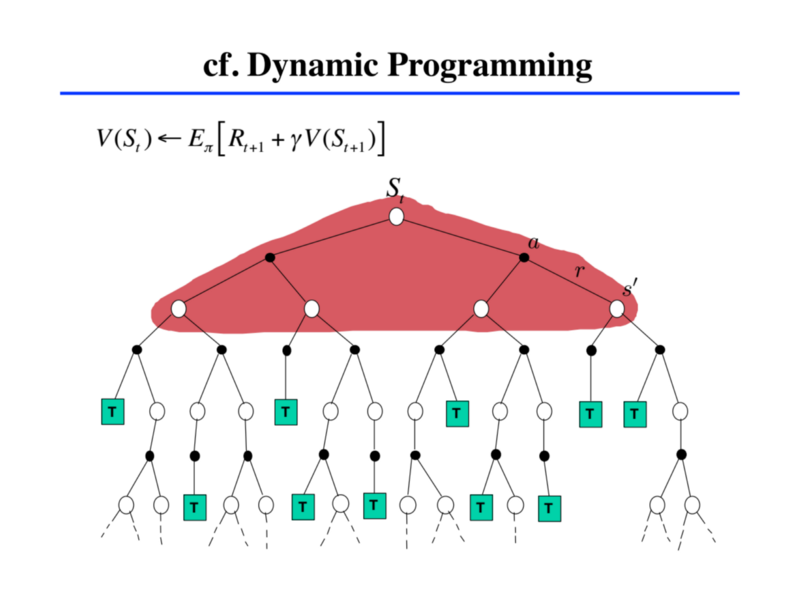
\includegraphics[height=.25\textheight, width=.5\textwidth]{dp.png}
			\item 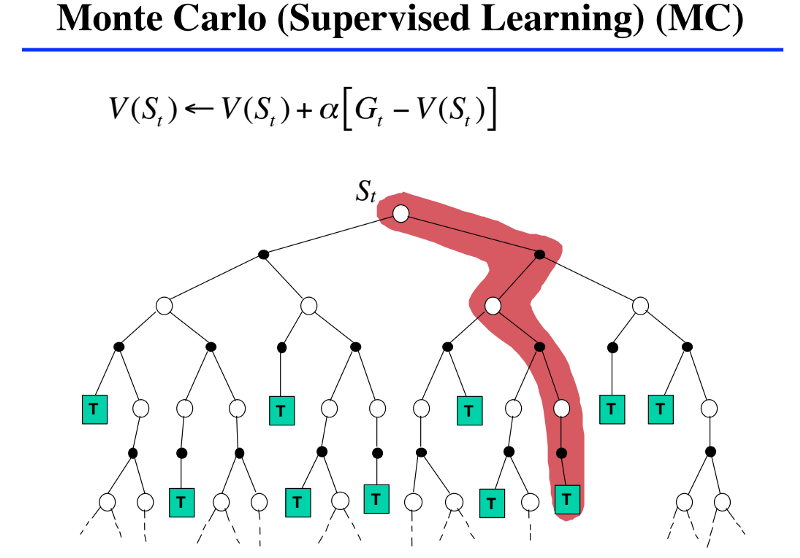
\includegraphics[height=.25\textheight, width=.5\textwidth]{mc.png}
			\item 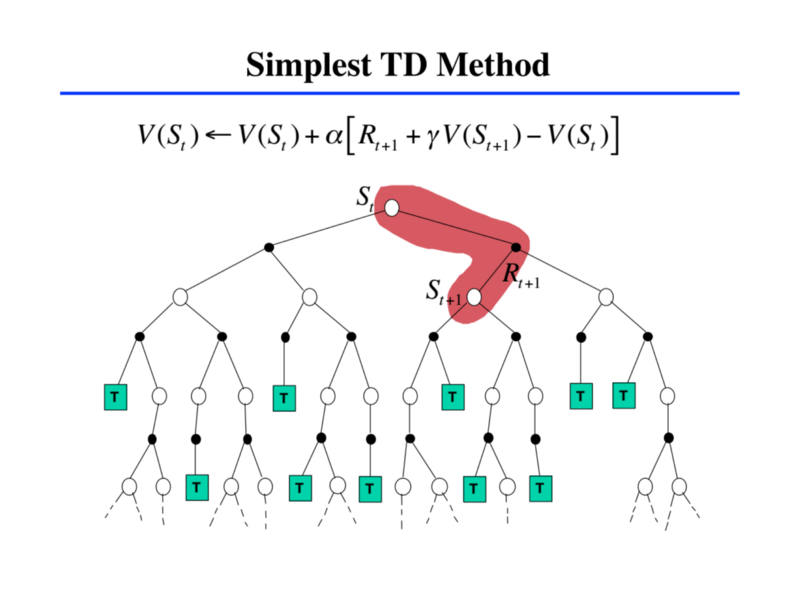
\includegraphics[height=.3\textheight, width=.5\textwidth]{td.png}

		\end{itemize}
    	%\includegraphics[<options, e.g. width=\textwidth>]{<your image file>}
    \end{block}
    \end{column}
\end{columns}

\end{frame}




\begin{frame}
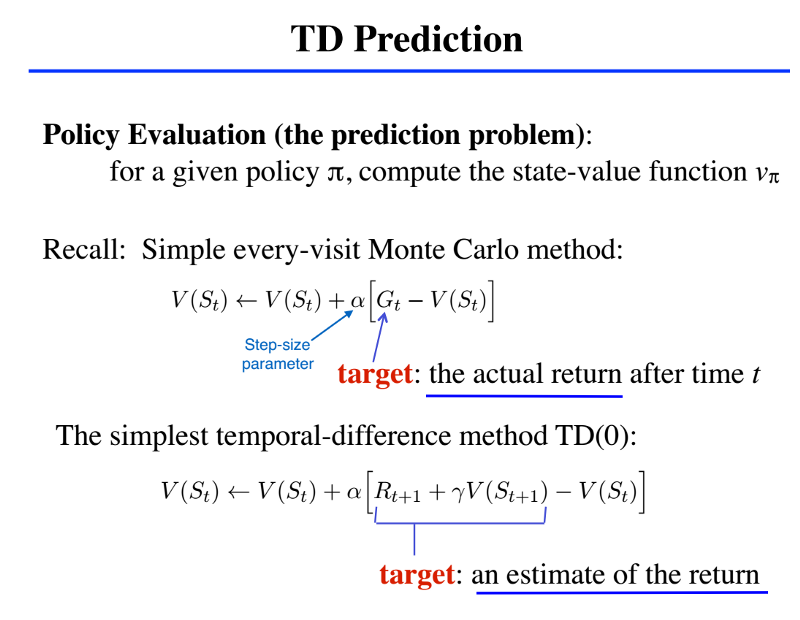
\includegraphics[height=\textheight, width=\textwidth]{tdPrediction.png}
\end{frame}

\begin{frame}
\frametitle{TD(0)}
\begin{itemize}
	\item  TD(0) or one step TD (update the value function after any individual step)
	\item  Only wait until the next time step to update the value estimates
	\item MC wait for full episode 
	\item 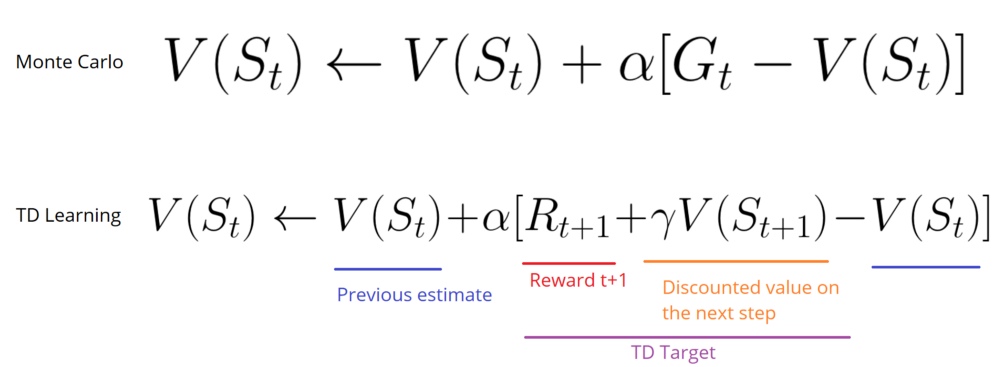
\includegraphics[height=.2\textheight, width=.6\textwidth]{mcVtd.png}
	\item More generalized TD($\lambda$) available in next chapters
\end{itemize}
				
\end{frame}

\begin{frame}
\frametitle{TD(0) Algorithm }
	\begin{itemize}
		\item Algorithm is
		\item 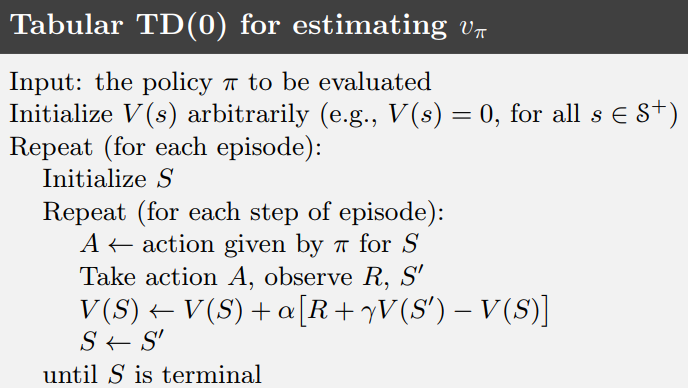
\includegraphics[height=.4\textheight, width=.4\textwidth]{tdZeroAlgo.png}
		\item Error at each step =  $R_{t+1}$ + $\gamma$ $V({S}_{t+1})$ - $V({S}_{t})$

	\end{itemize}
	
\end{frame}




\begin{frame}
\frametitle{Advantages of TD Prediction Methods)}
\begin{itemize}
	\item Do not require a model of the environment, only experience
	\item TD, but not MC, methods can be fully incremental
		\begin{itemize}
			\item You can learn before knowing the final outcome
			\item Do not wait for full episode
		\end{itemize}
	\item Less memory : Don't look all steps like DP
	\item Less peak computation
	\item Converges like MC : given certain assumptions 
	\item 
	
\end{itemize}

\end{frame}





\begin{frame}
\frametitle{Optimality of TD(0)}
Assume we have finite amount of experience : 10 episodes or 100 time steps for a Random Walk scenario
\begin{columns}
    \begin{column}{.6\textwidth}
     	\begin{block}{}
			\begin{itemize}
				
				\item Batch Update :
				\begin{itemize}
					\item time step $t$ : time to move to next step
					\item TD prediction equation: $V(S_t)  =  V(S_t)  + \alpha[R_{t+1} + \gamma   V(S_{t+1}) -  V (S_t)]$
					\item Increment = $\alpha[R_{t+1} + \gamma   V(S_{t+1}) -  V (S_t)]$
					\item At each $t$, increment is caculated \textbf{\textit{But}} $V(S_t) $ is updated after 100 steps
				\end{itemize}
				\item If $\alpha$ is small, under batch update $TD(0)$ converges to single answer
				\item MC also converges to single(but different ) answer 
			\end{itemize}
		\end{block}
    \end{column}
    \begin{column}{.4\textwidth}
    \begin{block}{}
	% Your image included here
		\begin{itemize}
			\item 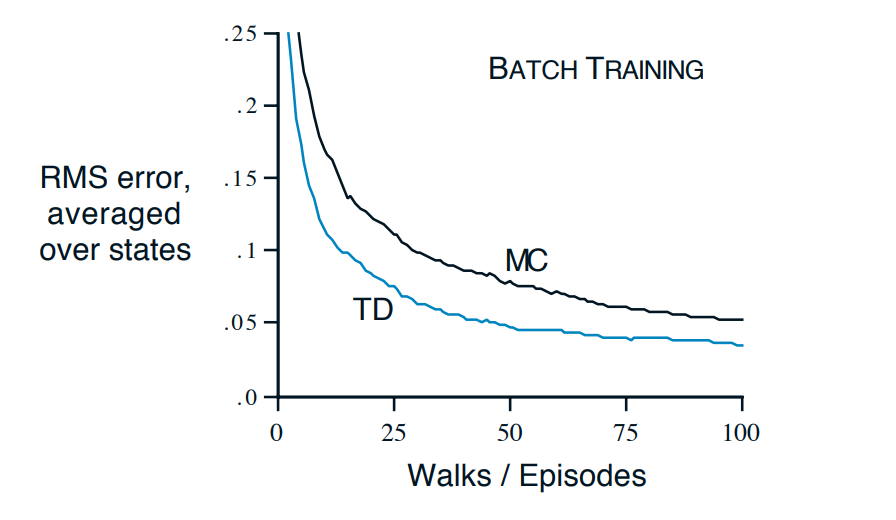
\includegraphics[height=.5\textheight, width=\columnwidth]{mctdoptimality.png}

		\end{itemize}
    	%\includegraphics[<options, e.g. width=\textwidth>]{<your image file>}
    \end{block}
    \end{column}
\end{columns}
			
\end{frame}


\begin{frame}
\frametitle{Performance of TD(0)}
\begin{itemize}
	
	\item Optimal solution requires : for $N$ states 
		\begin{itemize}
			\item $N^2$ memory \& $N^3$ computation
			\item Infesible for large problem
		\end{itemize}
	\item TD reaches to convergence faster than MC
		\begin{itemize}
			\item I am not clear about the logic !!!!
			\item certainty-equivalence estimate   -- I am not clear about that
		\end{itemize}
	\item For large state-space problem TD is only feasible solution
\end{itemize}

\end{frame}


\begin{frame}
\frametitle{On-policy / Off-policy}
\begin{itemize}
	\item On-Policy : 
	\begin{itemize}
		\item attempt to evaluate or improve the \textbf{\textit{policy($\pi $)}} used to make decisions
		\item Example :  SARSA
	\end{itemize}
	\item Of-Policy : 
	\begin{itemize}
		\item attempt to evaluate or improve the policy other than $\pi $
		\item Example :  Q-Learning
	\end{itemize}
\end{itemize}

\end{frame}







\begin{frame}
\frametitle{Sarsa: State-Action-Reward-State-Action}
\begin{columns}
    \begin{column}{.6\textwidth}
     	\begin{block}{}
			\begin{itemize}
				
				\item Simple TD : 
				\begin{itemize}
					\item Moves from $S_t$ to $S_{t+1}$
					\item Learns predicting optimal state 
					\item Action is defined by \textbf{\textit{Policy  $\pi$}}
					\item $\pi$ is not changed
				\end{itemize}
				\item On-Policy : 
					\begin{itemize}
						\item Changes $\pi$
						\item How:
						\begin{itemize}
							\item Instead of $S_t$ $\longrightarrow$ $S_{t+1}$ --- Do $Q(S_t, A_t)$ $\longrightarrow$ $Q(S_{t+1}, A_{t+1})$
							\item State action pair is learned $\longrightarrow$  $\pi$ is changed 
							\item Actions are updated $A \longrightarrow A'$ 

						\end{itemize} 
					\end{itemize}
				\end{itemize}
		\end{block}
    \end{column}
    \begin{column}{.4\textwidth}
    \begin{block}{}
	% Your image included here
		\begin{itemize}
			\item 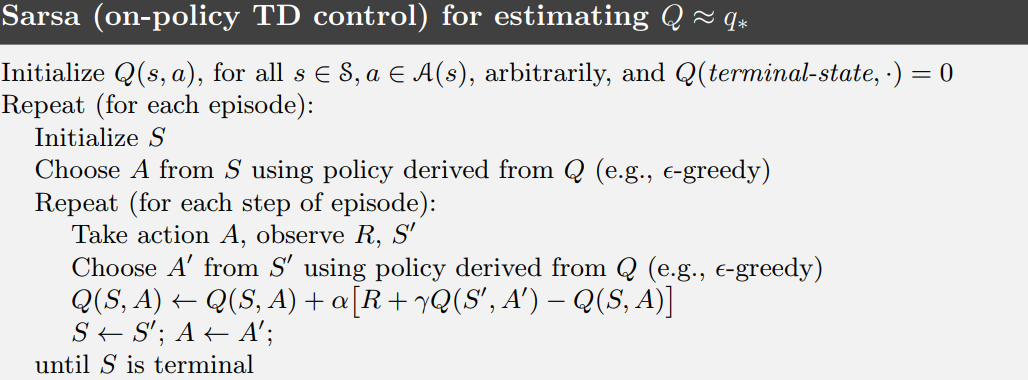
\includegraphics[height=.5\textheight, width=\columnwidth]{sarsa.png}

		\end{itemize}
    	%\includegraphics[<options, e.g. width=\textwidth>]{<your image file>}
    \end{block}
    \end{column}
\end{columns}
			
\end{frame}


\begin{frame}
\frametitle{Q-Learning: }
\begin{columns}
    \begin{column}{.6\textwidth}
     	\begin{block}{}
			\begin{itemize}
				
				\item Of-Policy : 
					\begin{itemize}
						\item Does not change $\pi$
						\item How:
						\begin{itemize}
							\item Instead of $S_t$ $\longrightarrow$ $S_{t+1}$ --- Do $Q(S_t, A_t)$ $\longrightarrow$ $Q(S_{t+1}, A_{t+1})$
							\item State action pair is learned $\longrightarrow$  $\pi$ is changed 
							\item Actions are \textbf{\textit{NOT}}  updated: NO $A \longrightarrow A'$  
						\end{itemize} 
					\end{itemize}
				\end{itemize}
		\end{block}
    \end{column}
    \begin{column}{.4\textwidth}
    \begin{block}{}
	% Your image included here
		\begin{itemize}
			\item 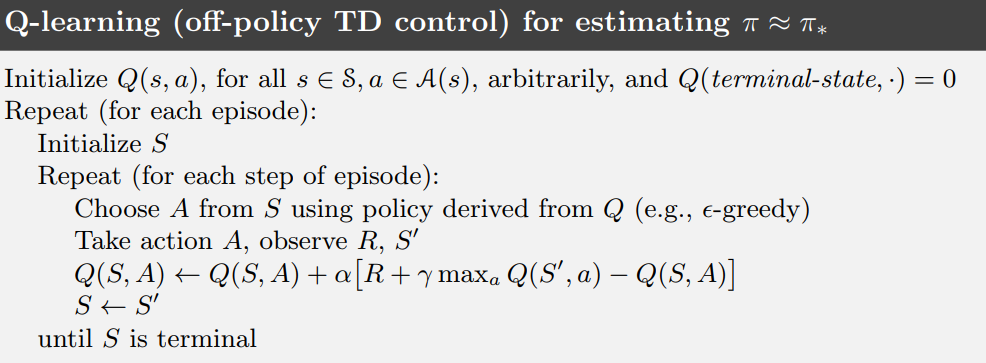
\includegraphics[height=.6\textheight, width=\columnwidth]{qlearning.png}

		\end{itemize}
    	%\includegraphics[<options, e.g. width=\textwidth>]{<your image file>}
    \end{block}
    \end{column}
\end{columns}
			
\end{frame}
\end{document}